\section{System Model}
In this section, we explain GPU task model on this paper while we discuss the gpu scheduling question and prior work.
Next, we make available limitation for clearing the implementation of no patched gpu scheduling.
This paper focus on a system composed of multiple GPU and multi-core CPU.

\subsection{GPU Task Model}
GPUを汎用的に利用する場合多くはCUDA、OpenCLが用いられる。
本稿ではCUDAに限定して記述するが、OpenCL等でも同様のアプローチが利用可能である。

GPU applications use a set of the API supported by the system,
typically talking the following steps.
(i) create GPU context (\textit{cuCtxCreate}), 
(ii) allocate space to device memory (\textit{cuMemAlloc}), 
(iii) The data and the GPU kernel are copied to the allocated device memory space from host memory (\textit{cuMemcpyHtoD}), 
(iv) Launch the GPU kernele (\textit{cuLaunchGrid}), 
(v) The GPU task is synchronized to the GPU kernel (\textit{cuCtxSynchronize}), 
(vi) The resultant data transfer to host memory from device memory (\textit{cuMemcpyDtoH}), 
(vii) release allocated memory space and context (\textit{cuMemFree, cuModuleUnload, cuCtxDestroy}).

我々は本稿においては、GPU実行が少しでも含まれるプロセスであり、ある事柄を成し遂げる一つの単位をアプリケーションとする。 (e.g. pedestrian detection application).
またこの一連の流れによってGPUを実行する1プロセスをGPUタスクとし、
GPU側で実行されるカーネルをGPUカーネルと定義する。

\subsection{Scheduling Discussion}
リアルタイムOSは古来より多くの研究\cite{spring,redline,itron,rk}が行われてきている。
LinuxをベースとしたリアルタイムOSとしても数多く研究\cite{prk,rtai,yodaiken1999rtlinux,litmus,kato:loadable}されている。
GPUを利用可能な環境はWindows, Mac OS, Linuxと限られており、リアルタイムという性質を追求するためにはLinuxの利用が最適であるため、今回我々はlinuxを利用する。

現在のシステムではGPUはI/Oデバイスとして利用される。
これまでに行われているRTOSに関する研究においても、
リソースカーネルなどでI/Oデバイスに関する研究は行われているが、
GPUをリアルタイムに扱うためには、これまでの知見だけでは不十分である。
これまでの一般的なディスクシステムなどのI/Oとの違いを以下にまとめる。

\begin{itemize}
\item データの送信、実行、データの受信と順序が固定されている且つそれぞれ独立した処理であること
\item ノンプリエンプティブであること
\item データ内容に依存しないため、複数のGPUが搭載された時に、どのGPUで実行してもよいこと
\end{itemize}

以上の特性はGPUをリアルタイム且つ効率的に利用するにあたり問題を複雑化させる。
具体的には、データの送受信、実行がオーバラップ可能なことで、スケジューリングが複雑化すること、ノンプリエンプティブによってオーバランを防ぐことが実質不可能であること、GPUへの自動割り当てや静的割り当てなど資源管理の複雑化が発生する。

加えてGPUタスクはデバイスな特性からSelf-suspending\cite{self-sus:1,self-sus:2}を発生させる。Self-suspensionなタスクにおけるスケジューリング解析については多くの研究がなされているが\cite{chattopadhyay2014limited,kim2013segment}、一般的な利用を行うためのハードルはあまりにも高い。

したがって、本誌ではまずはGPUをよりリアルタイムに扱うための環境を整えるために、
GPUタスクのスケジューリング且つ (マルチコア)、
GPUスケジューリングが可能な基盤を、
より簡易にインストールができ、より簡易にコンフィグ可能な形で提供する。

\textbf{Scheduling policies:}
ここでは上記スケジューリング基盤として備えるべきスケジューリングポリシーについて議論する。
CPU側で動作するタスクに関してはリアルタイムなシステムにおいては、優先度スケジューリング且ができていればよい。
固定優先度方式としてDeadline-Monotonic (DM)\cite{sched:dm}やRate-Monotonic (RM)\cite{sched:rm}などがあり、
動的優先度方式としてEarist deadline first (EDF) などがある。

GPUカーネルの実行に関しては優先度ベースなスケジューリングでは不都合が生じる。
GPUカーネルはGPUタスクに含まれるものである。
そのためGPUカーネルの優先度とGPUタスクの優先度が異なるケースは、その時点でGPUタスクの優先度逆転が発生する。
したがって、GPUカーネルスケジューリングは基本的にFIFOでスケジューリングすることが適正であり、それに加えて必要なのが各GPUタスクごとのGPUリクエストに対するQoSを担保することである。
QoSを担保する方法としてこれまでリソースリザベーションベースのスケジューリングポリシーが提案\cite{gdev,cbs,tbs}されてきており、
本論文ではGdevでGPUのQoS担保に一定の成果を挙げたBANDスケジューリングを利用する。

\textbf{No patched scheduler:}
To achieve "No patched", we must not to modify the kernel code and the device driver code.
RGEMはユーザスペースのみでGPUカーネルラウンチのスケジューリングを行っている。
GPUタスク間でPOSIXによって提供されるIPCを用いてタスク間の協調を行い、優先度ベースでのスケジューリングを実現している。
GPUのスケジューリングは同期ベースなスケジューリングを行うが、
RGEMでは同期の取得をランタイムに依存している。

同期の取得を行うように変更するためにカーネルスペースからのアプローチが必須である。
Gdevではカーネルスペースからのアプローチを行っているが、
同期の取得のためにカーネルへの変更を含んでいるため、
同期の取得をノーパッチで行うことが大きな課題である。

\textbf{GPU Synchronization:}
GPUを利用するシステムのようなヘテロジニアス且つメモリを共有しない場合に大きな課題となるのが同期である
GPUの同期は2つの手法がある。
一つはPollingを用いた方法で本誌ではFENCEと呼ぶ。
もう一つはInterruptによって同期する方法で本誌ではNOTIFYと呼ぶ。
これらは両者ともGPUに搭載されたエンジンを用いて行われる。
GPUには多くのエンジン(マイクロコントローラ)が搭載されている。
本論文では詳しいアーキテクチャはメインではないので省略するが、詳細は過去の文献\cite{kato:timegraph,fujii:apsys2013}に記載しています。
このエンジンにはコンテキスト管理用、コマンド受け取り用、データ転送用などが存在している。
通常、コマンド受け取り用のエンジンが受け取ったコマンドのヘッダから、
そのコマンドを使用するエンジンへと送信し、処理が行われる。
この順序はすべてFIFOで行われる。
FENCEを用いた方式では、まず同期用に仮想アドレス空間にマップされたバッファをGPUメモリに用意する。
そして、このメモリに値をEngine経由で書き込むためのコマンドを発行する。
Engineはカーネル実行とメモリ転送終了後に値を書き込むため、
CPU側でマップされたメモリアドレスをポーリングしながらチェックすれば同期が可能である。
NOTIFYについてもEngineの機能を利用する。
タスクはTASK\_INTERRUPTIBLE or TASK\_UNINTERRUPTIBLEにした上でschedule()を呼ぶか、
waitqueueなどを用いて上記に相当する処理を行いsuspendする。
そしてEngineから割込みを発生させるコマンドを発行し、割り込みコントローラがそれを獲得、
GPUドライバが登録した$Interrupt Service Routine$ (ISR) を立ち上げる。
ISR内では、各割込みに関するステータスをマッピングされたレジスタから読み込み、
各割込みごとに処理を行う。処理後は割込み完了フラグを書き込み、初期化する。
Gdevではsynchronization ベースのスケジューリングを行っており、GPUカーネル終了の検知し次のタスクを立ち上げる部分に割込みを用いている。

\begin{figure}[t]
\begin{center}
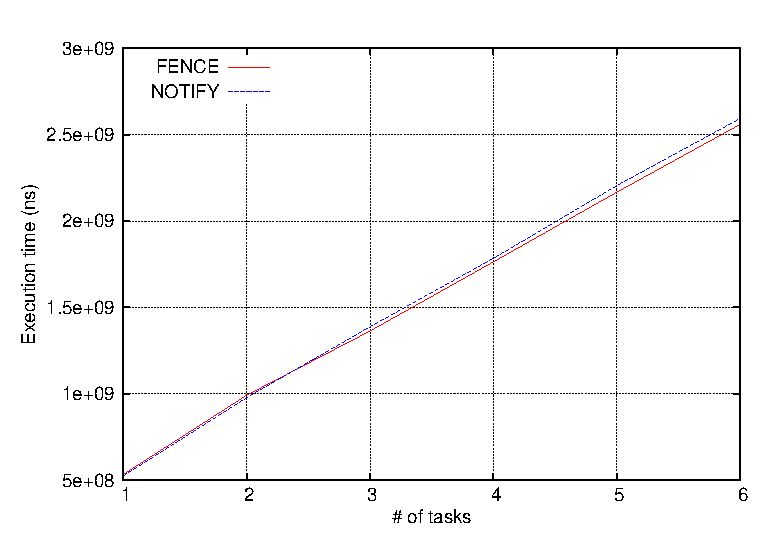
\includegraphics[width=0.35\textwidth]{img/poll_vs_irq}
\caption{FENCE vs NOTIFY}
\end{center}
\label{fig:poll_vs_irq}
\end{figure}

二種類の手法が存在する理由としては、FENCEとNOTIFYにそれぞれアドバンテージがあるためである。
Figure~\ref{fig:poll_vs_irq} shows FENCEを1とした時のNOTIFYのrelative speedである。
タスクが1つの場合はFENCEがNOTIFYよりも8ms速い結果が出ており、
タスクが3個に増えた時点でNOTIFYの方が早くなり、タスク6個の時点では33ms速い結果がでている。
NOTIFYによってタスクがスリープしている間に他のタスクのCPU利用部分が動作することで、
効率的にGPUタスクが実行できているためである。
GPUをより効率的に利用するためにはFENCE、NOTIFYをうまく使い分ける必要がある。

本稿で対象とするプラットフォームでは、複数のGPUタスクが存在し、複数のGPUカーネルが同一タスクに存在することを想定している。
そのため複数のGPUカーネルと一般的に同期に利用されるCUDA APIの$cuCtxSynchronize()$の回数は一対一で対応付けされずに、
複数のGPUカーネルの発行を一度の$cuCtxSynchronize()$によって同期する可能性がある。
そのため、$cuCtxSynchronize()$を用いた同期ベースなスケジューリングを行うにあたり、各GPUカーネルの終了と同期のために、アプリケーション自体の変更を必要とするため好ましくない。

本問題に対してGPUSyncではNOTIFYに限って対処しており、$LITMUS^{RT}$の拡張という形でLinuxの割込みのbottom-halfであるtaskletをカーネル内部で傍受し、
コールバック関数の引数のポインタが指すメモリスペースによって、どのGPUからの割込みかを判断している。
その手法では、soft-irqを利用しているためレイテンシが大きく、どのカーネルであるかの判断もできない。
GdevではGPUタスクの同期はFENCE、スケジューラの立ち上げはNOTIFYを用いている。
NOTIFYの獲得は、デバイスドライバがカーネルに登録するISRにGdevのコールバック関数を追記することで割込みタイミングを獲得している。
GPUタスクの同期にFENCEを用いている理由としては、あくまでGPUを効率よく扱う点にフォーカスしており、CPU側の処理も含めた効率について考慮していないためである。
カーネル、デバイスドライバの編集無しにスケジューリングするための最も大きな課題は、この同期を獲得し、識別するかといった点である。
